\documentclass{article}
% Use the following version of the ``usepackage'' statement for
% submitting the draft version of the paper for review.  This will set
% the note in the first column to ``Under review.  Do not distribute.''
\usepackage{icml2007} 
\usepackage{times} 
% Use this version of the ``usepackage'' statement after the paper has
% been accepted, when creating the final version.  This will set the
% note in the first column to ``Appearing in''
%\usepackage[accepted]{icml2007}
\usepackage{code}
\usepackage{url}
\usepackage{epsfig}
\usepackage{mlapa}
\newcommand{\cut}[1]{}

\newcommand{\appref}[1]{Appendix~\ref{#1}}
\newcommand{\secref}[1]{Section~\ref{#1}}
\newcommand{\tblref}[1]{Table~\ref{#1}}
\newcommand{\figref}[1]{Figure~\ref{#1}}
\newcommand{\listingref}[1]{Listing~\ref{#1}}
%\newcommand{\pref}[1]{{page~\pageref{#1}}}

\newcommand{\eg}{{\em e.g.}}
\newcommand{\cf}{{\em cf.}}
\newcommand{\ie}{{\em i.e.}}
\newcommand{\etc}{{\em etc.\/}}
\newcommand{\naive}{na\"{\i}ve}
\newcommand{\role}{r\^{o}le}
\newcommand{\forte}{{fort\'{e}\/}}
\newcommand{\appr}{\~{}}

\newcommand{\bftt}[1]{{\ttfamily\bfseries{}#1}}
\newcommand{\kw}[1]{\bftt {#1}}
\newcommand{\Pthen}{\kw{Pthen}}
\newcommand{\pads}{\textsc{pads}}
\newcommand{\padsl}{\textsc{padsl}}
\newcommand{\padst}{\textsc{pads/t}}
\newcommand{\datatype}{\textsc{PADS/T}}
%\newcommand{\datatype}{\textsc{DataType}}
\newcommand{\C}{\textsc{C}}
\newcommand{\perl}{\textsc{Perl}}
\newcommand{\ml}{\textsc{ml}}
\newcommand{\sml}{\textsc{sml}}
\newcommand{\smlnj}{\textsc{sml/nj}}
\newcommand{\java}{\textsc{java}}
\newcommand{\ddl}{\textsc{ddl}}
\newcommand{\xml}{\textsc{xml}}
\newcommand{\datascript}{\textsc{DataScript}}
\newcommand{\packettypes}{\textsc{PacketTypes}}
\newcommand{\erlang}{\textsc{Erlang}}

\newcommand{\Core}{Ad hoc}
\newcommand{\core}{ad hoc}
\newcommand{\pvalue}{\core{} value}
\newcommand{\ppat}{\core{} pattern}
\newcommand{\ptype}{\core{} type}

\newcommand{\padsc}{\textsc{pads}/\C{}}
\newcommand{\padsml}{\textsc{pads}/\ml{}}

\newcommand{\dibbler}{Sirius}
\newcommand{\ningaui}{Altair}
\newcommand{\darkstar}{Regulus}

\newcommand{\pdgood}{{\tt G}}
\newcommand{\pdbad}{{\tt B}}
\newcommand{\pdnest}{{\tt N}}
\newcommand{\pdsem}{{\tt S}}
\newcommand{\ptypes}{T}
\newcommand{\patreadpd}[2]{{\tt #1<<#2>>}}
\newcommand{\btm}{\cd{BOT}}


\newcommand{\lsem}{{[\![}}
\newcommand{\rsem}{{]\!]}}


\newcommand{\figHeight}[4]{\begin{figure}[tb]
	\centerline{
	            \epsfig{file=#1,height=#4}}
	\caption{#2}
	\label{#3}
	\end{figure}}

%% Environment for typesetting BNF grammars. Uses display math mode.
\newenvironment{bnf}
     {%% local command definitions:
        %% BNF definition symbol
      \def\->{\rightarrow}
%%      \def\::={{::=} &}
      \def\::={\bnfdef &}
      \def\|{\bnfalt}
      \newcommand{\name}[1]{\text{##1}}
        %% non-terminal
      \newcommand{\nont}[1]{{##1}}
      \newcommand{\meta}[1]{& ##1 &}
      \newcommand{\descr}[1]{& \text{// ##1}}
      \newcommand{\opt}[1]{ [##1] }
      \newcommand{\opnon}[1]{\opt{\nont{##1}}}
      \newcommand{\none}{\epsilon}
      \newcommand{\nwln}{\\ &&&}
      \newcommand{\nlalt}{\\ && \| &}
      \[\begin{array}{lrlll}
     }
     {\end{array}\]}

\newcommand{\mcd}[1]{\mathtt{#1}}
\newcommand{\ppair}[3]{#1{:}#2 \mathrel{**} #3}
\newcommand{\parray}[3]{#1\;\mcd{Parray}(#2,#3)}
\newcommand{\pset}[3]{\{#1{:}#2\,|\,#3\}}
\newcommand{\pstream}[1]{#1\;\mcd{stream}}
\newcommand{\precord}[1]{\{\{#1\}\}}

% The \icmltitle is too long. Therefore, a short form for the running title 
% is supplied just before \begin{document} 
%\icmltitlerunning{Submission and Formatting Instructions for ICML-2007}

\begin{document} 

\twocolumn[
\icmltitle{Towards 1-click Tool Generation with PADS}
]
\icmlauthor{David Burke and Peter White}{}
\icmladdress{Galois Connections}
\icmlauthor{Kathleen Fisher}{}
\icmladdress{AT\&T Labs}
\icmlauthor{David Walker and Kenny Q. Zhu}{}
\icmladdress{Princeton University}
% The following author list should only appear in the accepted versions. 
% \icmlauthor{Pat Langley}{langley@isle.org}
% \icmladdress{Institute for the Study of Learning and Expertise, 
%             2164 Staunton Court, Palo Alto, CA 94306 USA}
% \icmlauthor{Claude-Nicolas Fiechter}{fiechter@rtna.daimlerchrysler.com}
% \icmlauthor{Mehmet G\"{o}ker}{goker@rtna.daimlerchrysler.com}
% \icmladdress{DaimlerChrysler Research and Technology Center, 
%             1510 Page Mill Road, Palo Alto, CA 94304 USA}
% \icmlauthor{Cynthia Thompson}{cthomp@csli.stanford.edu}
% \icmladdress{Computational Learning Laboratory, 
%             Center for the Study of Language and Information, 
%             Stanford University, Stanford, CA 94305 USA}
% \icmlauthor{Andrea Danyluk}{andrea@cs.williams.edu}
% \icmladdress{Department of Computer Science, Williams College,
%             Williamstown, MA 01267 USA}
% \icmlauthor{Claude Sammut}{claude@cse.unsw.edu.au}
% \icmladdress{School of Computer Science and Engineering,
%             University of New South Wales,
%             Sydney NSW 2052, Australia}
% \icmlauthor{Tom Fawcett}{tom\_fawcett@hp.com}
% \icmladdress{HP Laboratories, 1501 Page Mill Road, 
%             Palo Alto, CA 94304 USA}
% \icmlauthor{Terran Lane}{terran@cs.unm.edu}
% \icmladdress{Department of Computer Science, University of New Mexico,
%             Albuquerque, NM 87131 USA}
% \icmlauthor{Jennifer Dy}{jdy@ece.neu.edu}
% \icmladdress{Department of Electrical and Computer Engineering, 
%             Northeastern University, 
%             Boston, MA 02115 USA}
% \icmlauthor{Dale Schuurmans}{dale@cs.ualberta.ca}
% \icmladdress{Department of Computing Science, University of Alberta, 
%              Edmonton, AB T6G 2E8 Canada}
% \icmlauthor{Kristian Kersting}{kersting@informatik.uni-freiburg.de}
% \icmladdress{Institute for Computer Science, University of Freiburg, 
%              Georges-Koehler-Allee, Bulding 079, 79110 Freiburg, Germany}
% \icmlauthor{Codrina Lauth}{Codrina.Lauth@ais.franhofer.de}
% \icmladdress{Fraunhofer Institute for Autonomous Intelligent Systems,
% 	     Schloss Birlinghoven, 53754 Sankt Augustin, Germany}
%]

%\begin{abstract} 
%ICML-2007 reviewing will be blind to the identities of the authors,
%and therefore identifying information should not 
%appear in papers submitted for review.
%\end{abstract} 

\section*{Introduction}
\label{intro}

An {\em ad hoc data source} is any semistructured data source
for which useful data analysis and transformation tools
have not yet been defined. XML, HTML and CSV are {\em not} 
ad hoc data sources as there are numerous programming libraries,
query languages, manuals and other resources dedicated to
helping analysts manipulate data in these formats.
However, ad hoc data does arise often in many fields including
computational biology, physics, finance, networking and 
systems administration.

The goal of the \pads{} project~\cite{padsweb} is to improve the
productivity of data analysts who need to deal with new and evolving
ad hoc data sources on a daily basis.  Our central technology is a
domain-specific language in which programmers can specify the
structure and expected properties of ad hoc data sources, whether they
be ASCII, binary, Cobol or a mixture of formats.  These
specifications, which resemble extended type declarations from
conventional programming languages, are compiled into a suite of
programming libraries and end-to-end data processing tools.  For
example, from any \pads{} description, our compiler can automatically
produce parser and printer libraries, a query engine, a format translator
and several others.

Unfortunately, it often takes substantial time, energy and expertise
to write a \pads{} description for a new ad hoc data source
-- days or even weeks for complex sources that have little or
no documentation, a common scenario in the world of ad hoc data.
Consequently, we have begun to study techniques for automatic
inference of \pads{} descriptions from example data, focusing for now
on ASCII data sources.   The rest of this 
short paper describes our preliminary efforts to do so.

% Our end
% goal is to provide users with an end system that allows them to
% automatically generate sufficiently accurate \pads{} descriptions 
% that these descriptions may be fed into our compiler to generate
% useful programming libraries and data 
% processing and visualization tools. 

% The goal of this project is to provide a generic framework that includes
% languages and tools to seamlessly automate data stream analysis. 
% Given some samples of the data stream, our prototype system produces 
% an intermediate
% representation of the structure of the data through structure discovery
% and refinement, and translates that representation into a
% declarative data-description language, \padsc{}. \padsc{} is 
% expressive enough to describe a variety of data feeds 
% including ASCII, binary, EBCDIC, Cobol, and mixed data formats.  
% From \padsc{}, a suite of tools can generated with functions for 
% parsing, manipulating, and summarizing the data. All these can be 
% done with a ``push of a button.''   


% Transactional data streams, such as sequences of stock-market buy/sell orders,
% credit-card purchase records, web server entries, and electronic fund
% transfer orders, can be mined very profitably.  As an example,
% researchers at AT\&T have built customer profiles from streams of
% call-detail records to significant financial effect~\cite{kdd99}.   
% Often such streams are high-volume: AT\&T's call-detail stream contains
% roughly 300~million calls per day requiring approximately 7GBs of
% storage space.  Typically, such stream data arrives ``as is'' in
% \textit{ad hoc} formats with poor documentation.  In addition, the
% data frequently contains errors.  The appropriate response to such
% errors is application-specific. 
% %Some applications can simply discard
% %unexpected or erroneous values and continue processing.  For other
% %applications, however, errors in the data can be the most interesting
% %part of the data.  

% Understanding a new data stream and producing a suitable parser are
% crucial first steps in any use of stream data.  Unfortunately, writing
% parsers for such data is a difficult task, both tedious and
% error-prone. It is complicated by lack of documentation, convoluted
% encodings designed to save space, the need to handle errors
% robustly, and the need to produce efficient code to cope with the
% scale of the stream.  Often, the hard-won understanding of the data
% ends up embedded in parsing code, making long-term maintenance
% difficult for the original writer and sharing the knowledge with
% others nearly impossible.

\section*{The PADS Language}
Before sketching the structure of our description inference techniques,
we explain the structure of the \pads{} specification language in greater
detail.  
% As mentioned in the introduction,
% \pads{} specifications are related to conventional type declarations,
% but compiled into parser and printer libraries and linked with
% generic program units that perform higher level tasks.  There
% actually two different specification languages, one for \C{} and
% one for \ocaml{}, but we restrict ourselves to discussion of the former.
As mentioned in the introduction,
\pads{} specifications are related to conventional type 
declarations.\footnote{Though there are two versions of \pads{},
one for \C{} and
one for \ocaml{}, we restrict ourselves to discussion of the \C{} version,
which should be more familiar to most readers.}  For example,
\pads{} has a number built-in base types for atomic items ranging
from integers of various kinds (\cd{Puint32} for a 32-bit unsigned integer;
\cd{Pint64} for a signed 64-bit integer), strings with different
termination conditions (\cd{Pstring(' ')} terminates on seeing a
space character) and more complex items such as 
 dates (\cd{Pdate}) and times (\cd{Ptime}).
To describe complex formats, \pads{} contains a number of type constructors
including \cd{Pstruct} and \cd{Parray} to describe sequences
of items in a file, and \cd{Punion}, \cd{Pswitch}, \cd{Penum} to 
describe various sorts of choices in a file.  Programmers
can also attach arbitrary constraints to descriptions.

As an example, consider the common log format for Web server logs.  A
typical record looks like the following:
% I deleted the -700 at the end of the date to make it fit on one line 
% properly...I assume it's OK to tell a white lie about the format...
{\small \begin{verbatim}
207.136.97.49 - - [15/Oct/2006:18:46:51] 
	"GET /tk/p.txt HTTP/1.0" 200 30
\end{verbatim}
}
This record contains the IP address of the requester, a pair of
dashes, the date and time of the request, the request string itself, 
a response code and the number of bytes transmitted.  A fragment of the
\pads{} description for such a data source follows.  
\begin{code}
\kw{Pstruct} webRecord \{
  Pip        ip;   " - - [";          
  Pdate(':') date; ":";
  Ptime(']') time; "]";     
  httpMeth   meth; " ";
  Puint8     code; " "; 
  Puint8     size; " "; \};

\kw{Parray} weblog \{ webRecord[] \};
\end{code}
This description gives a definition
for the {\tt weblog} type, which is a sequence (a {\tt Parray})
of arbitrarily many {\tt webRecord}s.  It also gives a definition
for the {\tt webRecord} type which includes an ip address, a date,
a time and some other items.  Notice, there are two sorts of fields
in the Web record structure, named fields (such as the field named
{\tt ip} with type {\tt Pip}) and unnamed fields (such as 
{\tt  " - - ["}).  The former hold data that programmers or generated
tools may access; the latter service syntactic separators read by
generated parsers and printed by generated printers.  The type
{\tt httpMeth} is another user-defined type not shown here.

% The auxiliary types \cd{http_method_t} and \cd{http_v_t} describes the various
% HTTP methods such as GET/PUT/LINK, and the version formats, respectively.
% The \cd{version} field is subject to a constraint predicate \cd{checkVersion}
% to ensure that obsolete methods such as \cd{LINK} and \cd{UNLINK} are only
% used with version HTTP/1.0.

% A number of tools can be generated in the form of a C library from the
% \padsc{} description. Some examples are: a parser that allows the user to
% parse the data stream into structured or semi-structure data such as
% comma-separated formats or XMLs; an accumulator tool that presents the user with 
% statistics of input data such as the frequency of each type appearing in
% the data, the accumulated error rate of each type declaration in the
% \padsc{} description; or a filter program that allows the users to specify
% some filtering condition and process the data to return on the information
% of interest to the users. 

% Now we would like to automatically generate \padsc{} descriptions base on
% sample data with minimum user intervention. To this end, 
% we propose an architecture to {\em infer} or ``learn'' \cite{higuera01current} 
% formats from ad hoc data samples and convert the formats to \padsc{}. 

\section*{The Inference Engine}
\begin{figure}
\begin{center}
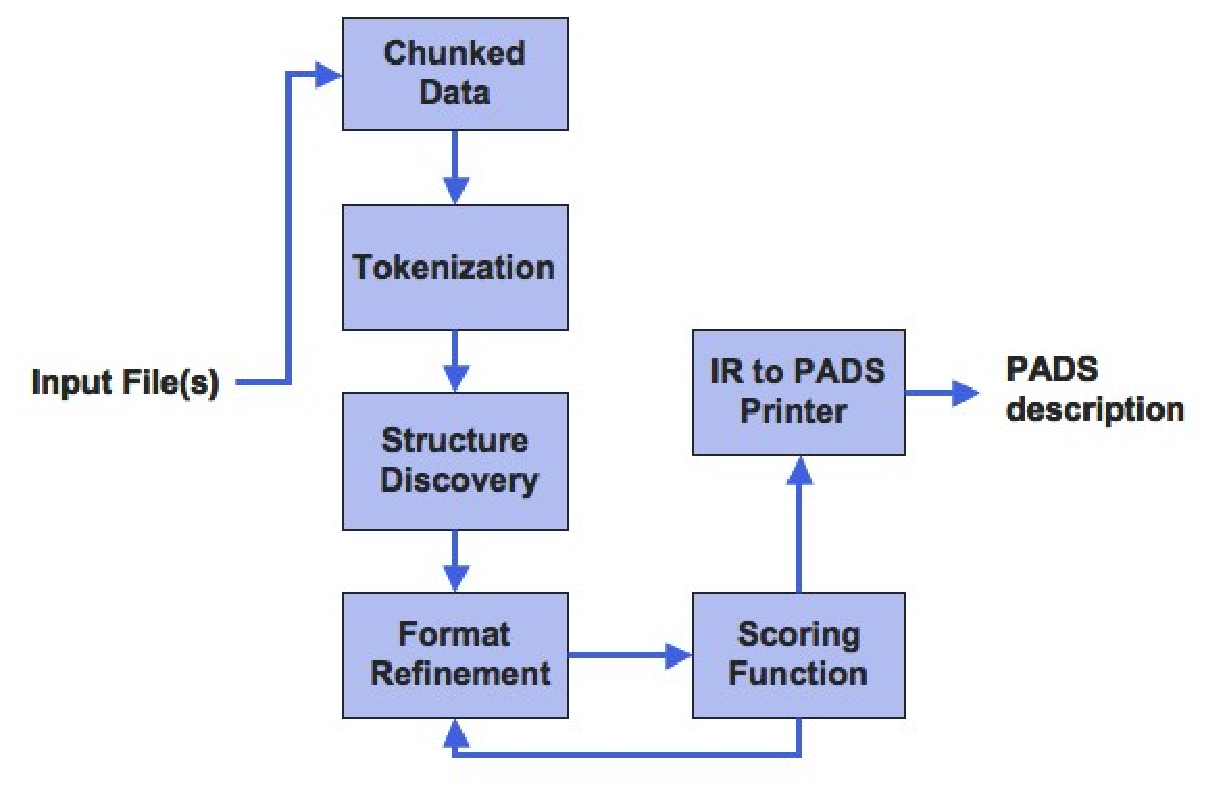
\epsfig{file=archi.eps, width=\columnwidth}
\caption{Architecture of the format inference engine}
\label{fig-archi}
\end{center}
\end{figure}
Figure \ref{fig-archi} gives an overview of our current format inference
architecture. The input data, or ``training set'', 
is first ``chunked'' into records where
each record is a piece of recurrent data such as a line, 
a paragraph, or a file (if the input consists of multiple files).
The unit of repetition is specified by the user when invoking our 
learning tool.
Each record is then broken down into a series of tokens where each
token can be a punctuation symbol, a number, a date, a time, or a number of other
basic types.  Our learning system has a basic tokenization scheme
skewed toward systems data, but users may specify a different scheme 
for their own domain through a configuration file that allows definition 
of new base types using regular expressions.  For example,
computational biologists may want to specify new base types for DNA strings
or other common recurring patterns.

In the structure discovery phase, we use a top-down, divide-and-conquer
scheme inspired in part by the work of Arasu on
information extraction from web pages~\cite{arasu+:sigmod03}. 
This scheme calculates
frequency distributions for tokens within records, and using this information,
chooses a simple type constructor such as a \kw{Pstruct}, \kw{Punion} or
\kw{Parray} to describe the top-level structure of the record. 
When a type is rector has been chosen, the data is partitioned accordingly
and the algorithm recursively analyzes subparts.  This
rough structure is represented in an intermediate representation (IR)
that has similar expressive power as the \pads{} language. 

The format refinement phase analyzes the IR produced by structure discovery
and repeatedly applies 
any one of a number of
rewrite rules.  There are two sorts of rewriting rules, 
value-independent rules
and the value-dependent rules.
The value-independent rules examine the inferred description structure,
and find ways to merge or rearrange components to improve the description.
Value-dependent rules analyze both the inferred description and the underlying
training data looking for fields for which the training data is constant
or one of a small number of values in order to introduce 
constant fields, enumerations.  The value-dependent rules also infer
certain kinds of inter-field dependency information.
At any given point during the refinement process,
many rewriting rules may apply -- our algorithm chooses the one 
that generates the description that optimizes an information-theoretic
scoring function we have defined.
The refinement step loops until there is no possible
improvement in the score. 
In effect, this refinement phase is equivalent to a greedy, local search
procedure aimming at improving the quality of the inferred format.
% The quality is measured by a scoring function which is based on the
% information theory. The objective of this function is to
% minimize the cost of transmitting the inferred format plus the
% training set. 
Below is a fragment of the IR learned from web log data similar to the data
illustrated above.  In this case, the learning system was quite successful,
though that is certainly not always the case.  The only mistake it
made was over specializing the response code 
to the specific integer constant 200.  It did so because the 
records in the training data contained no variation in this field.
{\small
\begin{verbatim}
Pstruct
  [IP];             [StringConst] " - - [";
  [Date];           [StringConst] ":";
  [Time];           [StringConst] "]";
  ...
  [IntConst] [200]; [StringConst] " " 
  [Pint];
End Pstruct
\end{verbatim}
}
Finally, after no more refinement is possible, the IR is translated
by a ``pretty printer'' into a working PADS 
specification,  which can be used to generate
a suite of useful tools.  In the case of our running example,
the learning system produces the specification fragment below.
{\small
\begin{verbatim}
Pstruct Struct_29 {
  Pip var_0; " - - [";
  Pdate(':') var_7; ':';
  Ptime(']') var_9; "] ";
  ...
  Puint8 var_26 : var_26 == 200; ' ';
  Pint64 var_28;
};

Parray entries_t { Struct_29[]; };
\end{verbatim}
}

\bibliography{main}
\bibliographystyle{mlapa}

\end{document} 
